\documentclass{beamer}
\usepackage[utf8]{inputenc}
% \usepackage[english]{babel}
\usepackage{hyperref}
\usepackage{graphicx}
\graphicspath{{../../../output/figures/Presentation/}}
\usepackage{wrapfig}
\usepackage{subcaption}
\usepackage{booktabs,bbm}
% \usepackage[square,numbers]{natbib}
%\bibliographystyle{unsrtnat}

\makeatletter
\let\@@magyar@captionfix\relax
\makeatother
\newtheorem{defn}[theorem]{Definition}
\DeclareMathOperator*{\argmax}{arg\,max}
\DeclareMathOperator*{\argmin}{arg\,min}
\hypersetup{
    allcolors={}
}

\usetheme{Boadilla}
\usecolortheme{beaver}

\usepackage[
backend=biber,
style=bwl-FU,
sorting=ynt
]{biblatex}
\addbibresource{main.bib}

\title[Agricultural Index Insurance]{Agricultural Index Insurance: An Optimization Approach}
\author[José Velarde Morales]{José I. Velarde Morales \and Linwei Xin}
\institute[Chicago Booth]
{

  University of Chicago\\
  Booth School of Business

}


\begin{document}
\beamertemplatenavigationsymbolsempty
\frame{\titlepage}
\section{Introduction}

\subsection{The Problem of Agricultural Risk}
\begin{frame}{The Problem of Agricultural Risk}
\begin{itemize}
    \setlength\itemsep{2em}
    \item Farmers face a lot of risk, and the lack of risk management tools forces them to use coping strategies that hurt their long term welfare.
   
    \item Traditional insurance is prohibitively costly in most developing countries due to lack of data and high verification costs.

    \item Moral hazard, adverse selection, and the presence of large covariate shocks make the problem of agricultural insurance especially hard. 
\end{itemize}
\end{frame}

\subsection{A Proposed Solution: Index Insurance}
\begin{frame}{A Proposed Solution: Index Insurance}
\begin{itemize}
   \setlength\itemsep{1em}
    % \item Researchers developed index insurance as a less costly way to offer insurance in developing countries. 
    \item In index insurance, an index (or statistic) is created using easily observable quantities (e.g. rainfall), and it is used to determine whether the insured party suffered an adverse event. 
    \item If the index falls below a pre-determined threshold, the insurance company automatically issues out payments to the insured. 
    \item This allows the insurance company to circumvent the issue of verification and moral hazard, since the actions of individual farmers cannot affect the index.
\end{itemize}
\end{frame}

\begin{frame}{Index Insurance in Practice}
\begin{itemize}
    \setlength\itemsep{1.5em}
    \item Since it was first proposed, index insurance programs have been implemented in many countries including India, Mexico, Tanzania, Malawi, Kenya, and many others (\cite{jensen2017agricultural}). 
    
    \item Today, tens of millions of farmers worldwide are covered by index insurance programs (\cite{greatrex2015scaling}). 
    
    \item However, in most of these cases, the insurance has to be heavily subsidized by governments due to high cost and low demand (\cite{greatrex2015scaling}). 
\end{itemize}
\end{frame}

\subsection{Project Overview}
\begin{frame}{Project Overview}
 \begin{itemize}
    \setlength\itemsep{1em}   
    \item Traditionally, contracts are designed to maximize correlation between payouts and losses. %This ignores valuable information about the correlation between zones that affects the cost of insuring the whole portfolio. 
    \item The goal of this project is to develop an optimization-based approach to contract design, that will allow us to include constraints.
    % \item Our method simultaneously determines the contract parameters for different areas, while taking into account the correlation between the areas, reducing risk for the insurer. 
    % \item This allows it to make better trade offs between coverage and the costs associated with risk.
 \end{itemize}
\end{frame}

% \begin{frame}{What I would like feedback on}
%     \begin{itemize}
%        \setlength\itemsep{1em}
%         \item Evaluation (what metrics to report, evaluation with observational and synthetic data, etc.)
%     \end{itemize}
%    \end{frame}

% \subsection{Literature Review}
\begin{frame}{Index Insurance Literature}
 \begin{itemize}
     \item \textbf{Impact of Index Insurance:} Overall, there is evidence that index insurance reduces reliance on detrimental risk-coping strategies, increases investment, and leads to riskier, but more profitable production decisions (\cite{jensen2017agricultural};  \cite{cole2013barriers}; \cite{mobarak2013informal}; \cite{karlan2014agricultural}).
     \item \textbf{Demand for Index Insurance:} Demand for index insurance tends to be low and highly price sensitive (\cite{jensen2017agricultural};  \cite{cole2013barriers}; \cite{cai2020subsidy},\cite{casaburi2018time}).
     \item \textbf{Design of Index Insurance:} There has been relatively little research studying the design of index insurance. The method developed by \cite{chantarat2013designing} is the most commonly used in academic publications (\cite{jensen2019does};  \cite{flatnes2018improving}). Recently, Chen et al 2023 developed a NN based method to design index insurance. 
    %  TODO: add chen paper
 \end{itemize}
\end{frame}

% \begin{frame}{Optimization Literature}
%  \begin{itemize}
%     \setlength\itemsep{2em}
%      \item We draw from the literature on chance constrained programs (\cite{lagoa2005probabilistically}; \cite{charnes1958cost}).
%      \item  We also draw on the work on coherent risk measures (\cite{artzner1999coherent}), and work on the optimization of conditional value at risk by (\cite{rockafellar2000optimization})
     
%      \item Additionally, we use the results on convex approximations of chance constrained programs by (\cite{nemirovski2007convex}).
%  \end{itemize}
% \end{frame}
\section{Background}
\begin{frame}[noframenumbering, plain]
    \frametitle{Content}
    \tableofcontents[currentsection]
  \end{frame}
\subsection{Index Insurance Background}
\begin{frame}{Three methods to design index insurance}
\begin{itemize}
    \setlength\itemsep{1em}
    \item Predict then optimize, choose contract that maximizes correlation between payouts and losses. No constraints. 
    \item End to end, use NN to design contracts, can handle few constraints. 
\end{itemize}
\end{frame} 

\begin{frame}{Index Insurance: Design}
% Index insurance design generally consists of three steps: 
\begin{enumerate}
    \setlength\itemsep{1em}
    \item Prediction: building a model to predict loss. 
    \item Contract design: designing contracts specifying payouts based on model predictions.
    \item Pricing: product pricing
\end{enumerate}
% This project focuses on the second step. Currently, a research team usually designs the insurance product, and the insurance company then prices the product.
\end{frame} 

\begin{frame}{Index Insurance: Definition and Parameters}
\begin{itemize}
    \setlength\itemsep{1em}
    \item Index insurance uses a signal, $\theta$, to predict agricultural loss, $\hat{\ell}(\theta)$
    \item Contract form: $I(\theta) = \min \left \{ \max \left \{a\hat{\ell}(\theta) - b,0 \right \}, 1 \right \}$, $a,b$ are the contract parameters.
    % \item Expected cost for insurer: $C(I(\theta)) = \mathbb{E}[I(\theta)] + c_{\kappa} K(I(\theta))$, where $c_{\kappa}$ is the cost of capital, and $K$ is required capital.
    % \item $K(I(\theta)) = CVaR_{1-\epsilon_P}\left ( I(\theta) \right ) - \mathbb{E}[I(\theta)]$.
\end{itemize}
\end{frame}

\begin{frame}{Example of Index Insurance Contract}
    \begin{figure}
        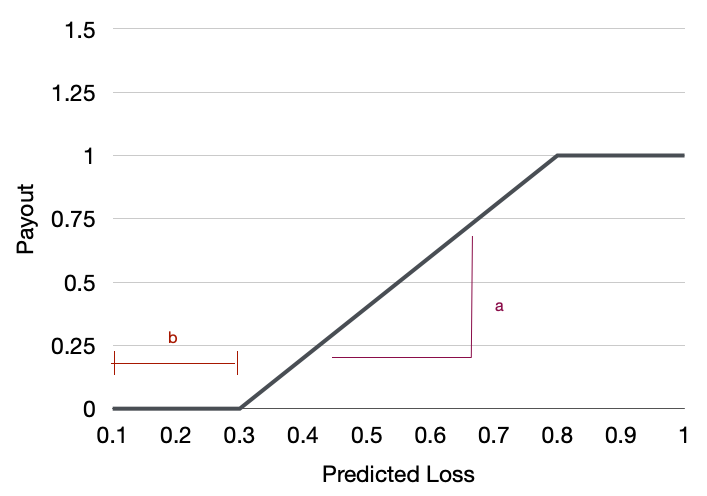
\includegraphics[width=0.9\textwidth]{../../../output/figures/Presentation/sample_insurance_contract.png}
    \end{figure}
\end{frame}

\section{Chen Framework}
\begin{frame}[noframenumbering, plain]
    \frametitle{Content}
    \tableofcontents[currentsection]
  \end{frame}

  
\begin{frame}{Model}
    Farmers start with wealth, $w_0$ and experience loss $\ell$. There is an index insurance contract $I$, that is determined by a $p$ dimensional vector of indices $\theta = (\theta_1,...,\theta_p)$. Premium for contract $I$ is $\pi(I)$. Farmer wealth is: 
    \begin{align*}
        w &= w_0 -\ell + I(\theta) -\pi(I)\\
        \pi(I) &= \lambda \mathbb{E}[I(\theta)]
    \end{align*}
\end{frame}

\begin{frame}{Optimization Problem}
    They solve the following optimization problem: 
    \begin{align}
        \max_{I \in \mathcal{I}}  & \quad \mathbb{E} \left [ U \left ( w_0 - \ell - \pi + I(\theta) \right ) \right ]\nonumber \\
        \text{s.t.} & \quad \underline{\pi} \leq \pi(I) \leq \overline{\pi}\\
        & \quad \pi = \lambda \mathbb{E}\left [ I(\theta) \right ] \\
        & \quad U \left (w \right ) = -(1/\alpha)e^{-\alpha w} 
    \end{align}
\end{frame}

\begin{frame}{Solution and results}
    \begin{itemize}
       \setlength\itemsep{2em}
        \item They use a neural network to solve the optimization problem. 
        \item Network they use has $\sim 10,000$ parameters. 
        \item They test it on Illinois corn yield data and find that the contracts are utility improving on average.  
        \item Their method is end-to-end, it goes directly from weather variables to payouts. 
    \end{itemize}    
    \end{frame}

\begin{frame}{Drawbacks}
    \begin{itemize}
        \setlength\itemsep{2em}
        \item Not interpretable, can't set constraints on variables that policy makers might care about (e.g. deductible).
        \item Model requires a lot of data to train, the data they tested the model on went back to 1925, unrealistic for developing countries. 
        \item Definition of premium used depends only on expected value of the payout and not on variance of the payouts, in practice the price would depend on riskiness of contract. 
    \end{itemize}    
    \end{frame}

\section{Optimization Approach}

\subsection{Prediction}
\begin{frame}{Overview}
    \begin{itemize}
        \setlength\itemsep{2em}
        \item We opt for a "predict-then-optimize" approach.
        \item We use specialized time-series feature extraction algorithms for feature extraction and traditional ML algorithms (e.g. Random Forest, Gradient Boosting, Support Vector Machines)
        \item These algorithms require less data to train.
    \end{itemize}
\end{frame}

\subsection{Model}
\begin{frame}{Model}
    We use the same model, just a different definition of the premium. 
    \begin{itemize}
        \setlength\itemsep{2em}
        \item Premium: $\pi(I(\theta)) = \mathbb{E}[I(\theta)] + c_{\kappa} K(I(\theta))$, where $c_{\kappa}$ is the cost of capital, and $K$ is required capital.
    \item $K(I(\theta)) = CVaR_{1-\epsilon_P}\left ( I(\theta) \right ) - \mathbb{E}[I(\theta)]$.
    \end{itemize}
    I got this definition from \textit{Risk Modeling for Appraising Named Peril Index Insurance Products: A Guide for Practitioners} (\cite{mapfumo2017risk}). The EU's Solvency requirements are similar. 
    % \item Expected cost for insurer: $C(I(\theta)) = \mathbb{E}[I(\theta)] + c_{\kappa} K(I(\theta))$, where $c_{\kappa}$ is the cost of capital, and $K$ is required capital.
    % \item $K(I(\theta)) = CVaR_{1-\epsilon_P}\left ( I(\theta) \right ) - \mathbb{E}[I(\theta)]$.
\end{frame}

\begin{frame}{Idealized Model}
\label{ideal-model}

 
\begin{align}
    \max_{a,b,\pi, K}  & \quad \mathbb{E} \left [ U\left ( w_0 - \ell - \pi + I(\theta) \right ) \right ] \label{cons-objective}\\
    \text{s.t.} & \quad I(\theta) =  \min \left \{\max \left \{0,a\hat{\ell}(\theta) + b \right \}, 1 \right \}\label{cons-contract}\\
    & \quad \pi = \mathbb{E}\left [ I(\theta) \right ] + c_{\kappa} \left[ {\sf CVaR}_{1-\epsilon_K}\left ( I(\theta)\right )  - \mathbb{E}[I(\theta)]  \right] \\
    % & \quad \underline{f} \leq \mathbb{P}\left ( I(\theta) > 0 \right ) \leq \overline{f} \label{cons-frequency}\\
    &\quad \pi \leq \overline{\pi}.\label{cons-capital}
\end{align}
\end{frame}

\begin{frame}{Convex Relaxation}

    We use the following convex and concave relaxations of $I(\theta)$: 
    \[
    \overline{I(\theta)} \triangleq\ \max \left \{ 0,a\hat{\ell}(\theta) + b\right \},\ \ \ \ 
    \underline{I(\theta)} \triangleq\ \min \{ a\hat{\ell}(\theta) + b,1 \}.
    \]
    Note that $\overline{I(\theta)}$ is convex in $\hat{\ell}(\theta)$, $\underline{I(\theta)}$ is concave in $\hat{\ell}(\theta)$, and
    \begin{align*}
    \underline{I(\theta)} \leq\ I(\theta) \leq\ \overline{I(\theta)}.
    \end{align*}
 We replace $I(\theta)$ in Problem \eqref{cons-objective} with either $\overline{I(\theta)}$ or $\underline{I(\theta)}$ where necessary to obtain a conservative and convex relaxation. 
% \hyperlink{ideal-model}{\beamerbutton{Idealized model}}\\
% \hyperlink{convex-approx}{\beamerbutton{Convex approximations}}
\end{frame}

\begin{frame}{Convex Relaxation}
    \begin{align}
        \max_{a,b,K,\pi} &\quad \mathbb{E} \left [  U\left(w_0 - \ell - \pi  +  \underline{I(\theta)} \right) \right ]\label{eq-06}\\
        \text{s.t.} & \quad \overline{I(\theta)} = \max \left \{0,a\hat{\ell}(\theta) + b \right \} \nonumber\\
        & \quad \underline{I(\theta)} = \min \left \{a\hat{\ell}(\theta)+b,1 \right \} \nonumber\\
        & \quad \pi = \left (1-c_{\kappa} \right ) \mathbb{E} \left [ \overline{I(\theta)} \right ] + c_{\kappa} {\sf CVaR}_{1-\epsilon_K} \left( \overline{I(\theta)} \right) \label{eq-41}\\
        % & \quad a \hat{F}^{-1}(\overline{f}) \leq b \leq a\hat{F}^{-1}(\underline{f})\\
        & \quad \pi \leq \overline{\pi} \nonumber.
  \end{align}
    
\end{frame}



\begin{frame}{CP Reformulation}
\scalebox{0.7}{\parbox{\linewidth}{%
Using the results from \cite{rockafellar2002conditional}, we get: 
    \begin{align*}
        \max_{a,b,\alpha,\omega,\gamma,t_K,K,\pi} \quad & \frac{1}{N} \sum_j \sum_z U\left ( w_{0,z} -\ell_z^j -\pi_z + I_z(\theta^j_z) \right ) \\
        \text{s.t.} \pi_z &= \left (1-\frac{c_{\kappa}}{\sum_z s_z} \right ) \frac{1}{N} \sum_j \alpha^j_z + \frac{c_{\kappa}}{\sum_z s_z}  \left (K - \frac{1}{N} \sum_j \sum_{z' \neq z} s_{z'} \omega_{z'}^j \right )\\
        t_K &+ \frac{1}{\epsilon_K} \sum_j p^j \gamma_K^j \leq K\\
        \gamma_K^j &\geq \sum_z s_z \alpha^j_z -t_K, \forall j \\
        \gamma_K^j &\geq 0, \forall j\\
        \alpha^j_z &\geq a_z \hat{\ell_z}(\theta^j_z) + b_z, \forall j, \forall z\\
        \alpha^j_z &\geq 0, \forall j, \forall z\\
        \omega^j_z &\leq a_z \hat{\ell_z}(\theta^j_z) + b_z, \forall j, \forall z\\
        \omega^j_z &\leq 1, \forall j, \forall z\\
        % a_z\hat{\ell_{z}^{\underline{f}}} &\leq b_z\\
        % a_z\hat{\ell_{z}^{\overline{f}}} &\geq b \\
        \pi_z &\leq \overline{\pi_z}, \forall z.
      \end{align*}
    }}
\end{frame}



\section{Evaluation}
\subsection{Data}
\begin{frame}{Data}
    Used two main data sources
    \begin{itemize}
        \setlength\itemsep{2em}
        \item Illinois annual corn yield data from the National Agricultural Statistics Service (NASS). Data is available at the county level from 1925-2022. 84 counties. 
        \item Weather data from the PRISM climate group. Has monthly data on several weather variables (temperature, precipitation, etc). Available 1895-present.
    \end{itemize}
\end{frame}

\subsection{Procedure}
\begin{frame}
    \begin{itemize}
        \setlength\itemsep{2em}
        \item We use a 70/15/15 train/val/test split. Data is kept in chronological order. Training data has older years and test data has the newest years. 
        \item We modified Chen's method to use the same definition of the premium as our method. 
        \item We use the training and validation data to design the contracts using both methods, apply the contracts to farmers in the test set, and compute performance metrics. 
    \end{itemize}
\end{frame}


\subsection{Results}
\begin{frame}{Overview}
    \begin{itemize}
        \item No method really dominates the other. 
        \item Generally, whichever method costs more tends to have higher utility for farmers. 
        \item In terms of farmer utility, our method tends to work better with realistic data lengths. 
    \end{itemize}
\end{frame}

\begin{frame}{Data Shortening}
    \begin{figure}
        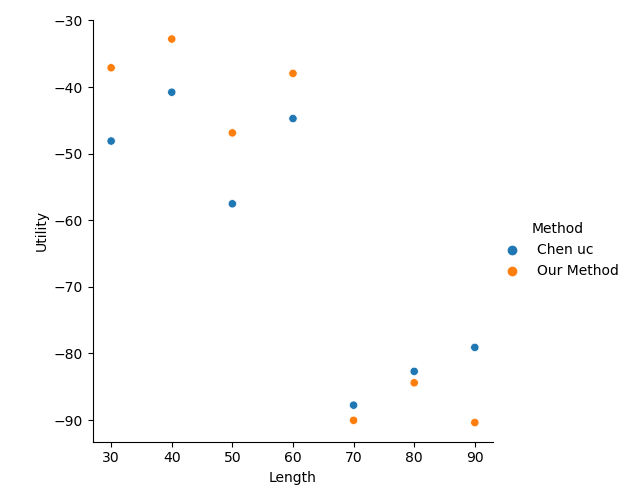
\includegraphics[width=0.75\textwidth]{../../../output/figures/Chen_Replication/Our_premium_results.png}
    \end{figure}
\end{frame}

\begin{frame}{Farmer Wealth distribution: 45 years of data}
    \begin{figure}
        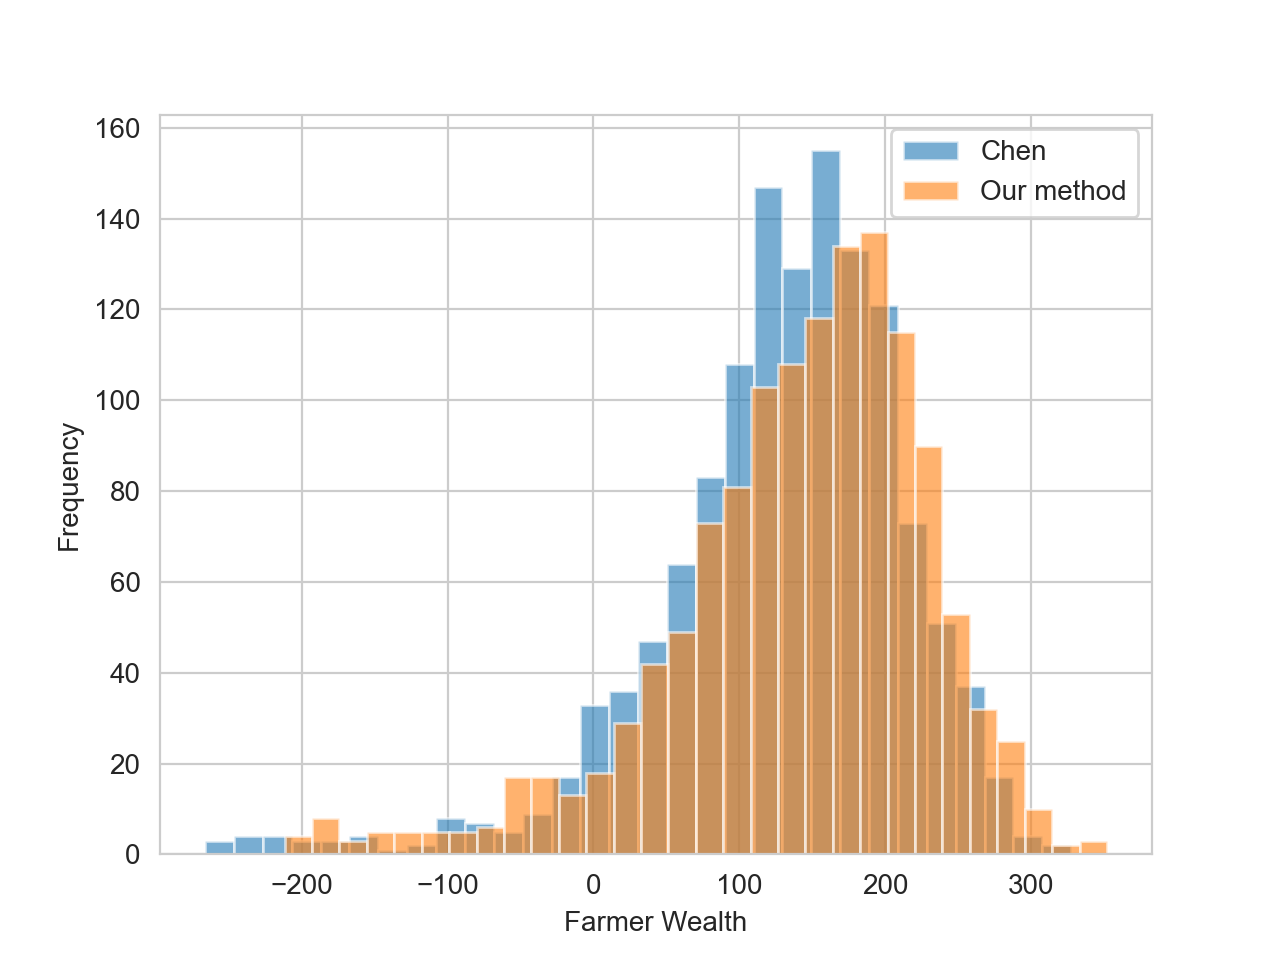
\includegraphics[width=0.75\textwidth]{../../../output/figures/Chen_Replication/farmer_wealth_hist2.png}
    \end{figure}
\end{frame}

\begin{frame}{Payouts vs Losses}
    \begin{figure}
        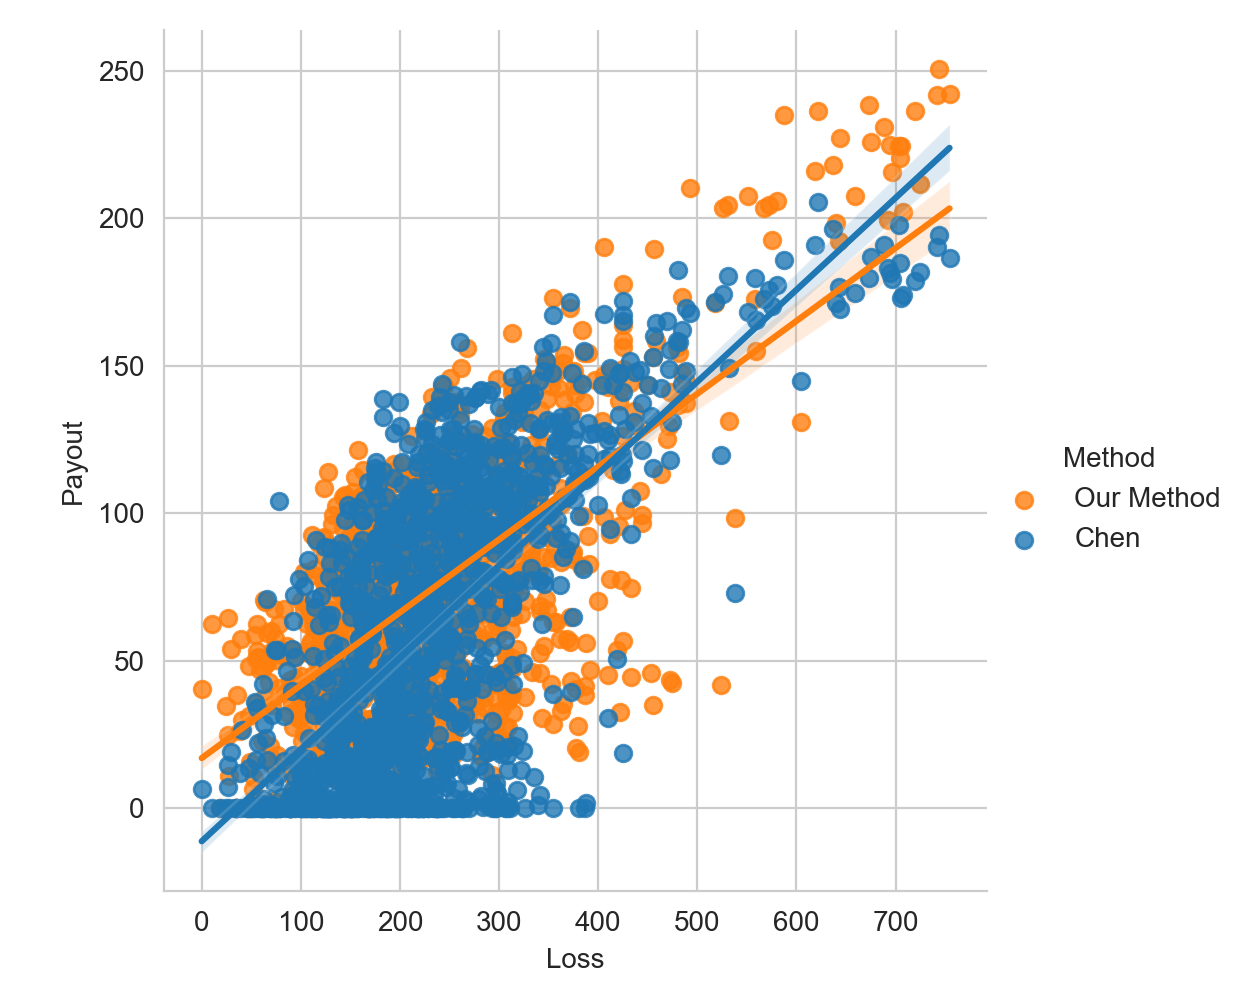
\includegraphics[width=0.75\textwidth]{../../../output/figures/Chen_Replication/combined_scatter.png}
    \end{figure}
\end{frame}

\begin{frame}{Multiple Zone}
    \begin{align}
        \max_{a,b,K,\pi} &\quad \mathbb{E}\left [ \sum_z U\left ( w_{0,z} -\ell_z^j -\pi_z + I_z(\theta^j_z) \right ) \right ]\label{eq-33}\\
        \text{s.t.} &\quad \pi_z  = \mathbb{E}\left [ \overline{I_z(\theta_z)} \right ] + \frac{c_{\kappa}}{\sum_z s_z}  K\\
        &\quad K = {\sf CVaR}_{1-\epsilon_K} \left ( \sum_z s_z\overline{I_z(\theta_z)} \right ) - \mathbb{E}\left [ \sum_{z} s_{z}\underline{I_{z}(\theta_{z'})} \right ] \label{eq-32}\\
        % & \quad a_z\hat{\ell_{z}^{\underline{f}}} \leq b_z \leq a_z\hat{\ell_{z}^{\overline{f}}}\\
        &\quad \overline{I_z(\theta_z)} = \max \left \{0,a_z\hat{\ell_z}(\theta_z) + b_z \right \} \nonumber\\
        &\quad\underline{I_z(\theta_z)} = \min \left \{a_z\hat{\ell_z}(\theta_z)+b_z,1 \right \} \nonumber\\
        &\quad\pi_z \leq \overline{\pi_z} \nonumber.
      \end{align}
    
\end{frame}

\begin{frame}{Next steps}
    \begin{itemize}
        \setlength\itemsep{2em}
        \item Compare the cost of insuring the US midwest
    \end{itemize}
\end{frame}












\section{Conclusion and Next Steps}
\subsection{Conclusions}
\begin{frame}{Conclusions}
    \begin{itemize}
    \setlength\itemsep{2em}
        \item The contracts designed by our model are able to offer better protection at a similar costs, or comparable protection at lower costs than the baseline method. 
        \item It outperforms the baseline when the prediction model is incorrectly specified and on the Kenyan pastoralist data. 
        \item Our method is more cost effective because it takes into account spatial correlations between  areas and the costs of capital requirements. Thus, the model makes better trade offs between costs and coverage than the baseline method. 
        
    \end{itemize}
\end{frame}

% \subsection{Next Steps}
% \begin{frame}{Next Steps}
% \begin{itemize}
% \setlength\itemsep{2em}
%     \item We are working with practitioners to improve the model and possibly test it in practice.
%     \item We are working with the Bank of Thailand on the implementation of their satellite-based index insurance program. 
%     \item We are also talking to the International Research Institute for Climate and Society at Columbia, they have worked on the implementation of numerous index insurance programs in Africa.   
% \end{itemize}
% \end{frame}

\begin{frame}[noframenumbering, plain]{References}
\printbibliography
\end{frame}

\begin{frame}[noframenumbering, plain]{Idealized CVaR Model}
% \label{ideal-model}
\begin{itemize}
    \item \textbf{Objective:} conditional value at risk of the farmers' loss net of insurance.
    \item  \textbf{Constraint 1:} piecewise linear structure of the contract. 
    \item \textbf{Constraint 2:} budget constraint.
    \item \textbf{Constraint 3:} definition of required capital.
\end{itemize}
 
\begin{align}
        \min_{a,b,\pi, K}  & \quad CVaR_{1-\epsilon}\left ( \ell - I(\theta) \right ) \notag\\
        \text{s.t.   }I(\theta) &= \min \{ (a\hat{\ell}(\theta) + b)^+,P \} \\
        \mathbb{E}\left [ I(\theta) \right ] &+ c_{\kappa} K \leq B \\
        K &= \left( CVaR_{1-\epsilon}\left ( I(\theta) \right ) - \mathbb{E}[I(\theta)] \right) \label{cons-budget}
    \end{align}
\end{frame}

\begin{frame}[noframenumbering, plain]{The problem is non-convex, so we need convex approximations}
\label{convex-approx}
We use the following approximations of $I(\theta)$ to make the problem convex: 
\begin{align*}
    \overline{I(\theta)} &\triangleq \max \left \{ 0,a\hat{\ell}(\theta) + b\right \} \\
    \underline{I(\theta)} &\triangleq \min \{ a\hat{\ell}(\theta) + b,K \}
\end{align*}
\begin{itemize}
    \item Note that $\overline{I(\theta)} \geq I(\theta)$ and $\overline{I(\theta)}$ is convex. Conversely, $\underline{I(\theta)} \leq I(\theta)$ and $\underline{I(\theta)}$ is concave. 
    \item We replace $I(\theta)$ with either $\overline{I(\theta)}$ or $\underline{I(\theta)}$ where necessary to obtain conservative and convex approximations. 
    \item We also need approximations or proxies for $E[I(\theta)]$ in constraint . We use $\pi_{SQ} = E[I_{SQ}(\theta)]$, where $I_{SQ}$ is the contract designed using the status quo method, as a proxy for $E[I(\theta)]$ in constraint .
\end{itemize}
\end{frame}

\begin{frame}[noframenumbering, plain]{Insights: Relationships between parameters and epsilon}
\label{eps-relationship}
As $\epsilon$ gets smaller, the slope increases and the function shifts to the right. 
\begin{figure}
\centering
  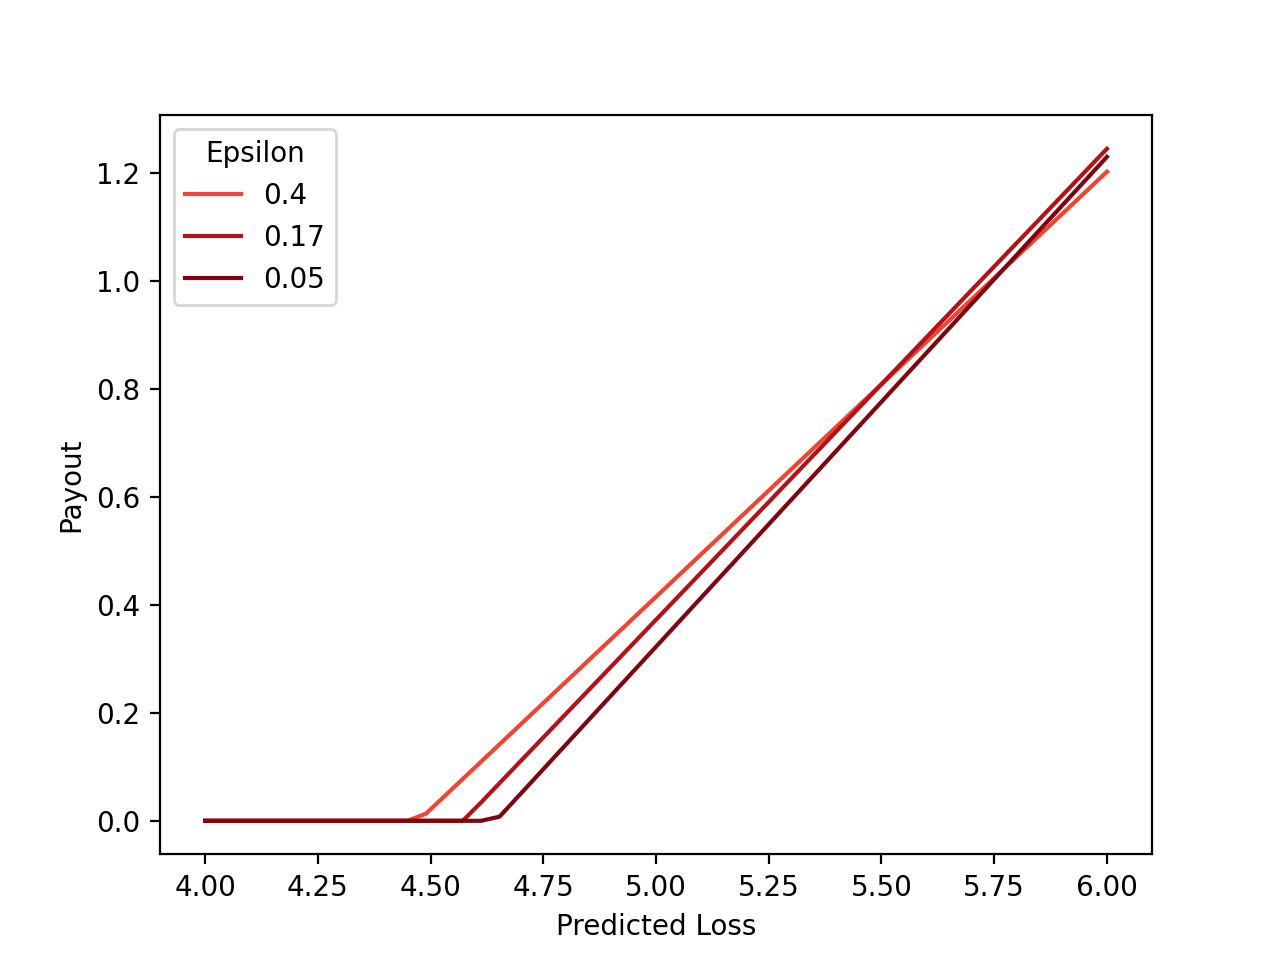
\includegraphics[width=0.65\textwidth, height=0.5\textwidth]{payout_vs_epsilon.png}
\end{figure}
    
\end{frame}

\begin{frame}[noframenumbering, plain]{Results: Misspecified Prediction Model}
\label{misspec-results}
\fontsize{6.5pt}{8pt}\selectfont
\begin{table}
\subcaptionbox{No correlation}{
\begin{tabular}{ccccc}
\toprule
   Model &        Max VaR & $|VaR_2 - VaR_1|$ & Required Capital &   Average Cost \\
\midrule
Baseline &          27.42 &              1.65 &            53.85 &          40.73 \\
         & [25.13, 29.57] &      [0.16, 5.56] &   [44.81, 59.88] & [36.06, 45.83] \\
     Opt &          27.41 &              1.96 &            49.97 &          40.36 \\
         & [24.53, 29.83] &       [0.15, 5.6] &   [42.87, 58.53] &  [35.52, 45.5] \\
\bottomrule
\end{tabular}}

\subcaptionbox{Positive correlation}{
\begin{tabular}{ccccc}
\toprule
   Model &        Max VaR & $|VaR_2 - VaR_1|$ & Required Capital &   Average Cost \\
\midrule
Baseline &          27.16 &              1.23 &             57.1 &          41.36 \\
         &  [24.7, 29.62] &       [0.1, 5.05] &    [51.16, 62.9] & [36.24, 46.52] \\
     Opt &          27.71 &               1.1 &            56.51 &          41.31 \\
         & [24.91, 30.31] &      [0.09, 3.62] &   [50.92, 62.26] & [35.98, 46.82] \\
\bottomrule
\end{tabular}}

\subcaptionbox{Negative correlation}{
\begin{tabular}{ccccc}
\toprule
   Model &        Max VaR & $|VaR_2 - VaR_1|$ & Required Capital &   Average Cost \\
\midrule
Baseline &          27.52 &               1.9 &             25.2 &          36.42 \\
         & [25.09, 29.69] &       [0.17, 6.0] &   [17.99, 36.35] & [33.13, 41.88] \\
     Opt &          27.39 &              1.84 &            26.77 &          36.67 \\
         & [24.33, 29.71] &      [0.16, 5.49] &    [18.17, 37.5] & [33.21, 42.03] \\
\bottomrule
\end{tabular}
}
\end{table}
\end{frame}

\end{document}